\section{Recap}
\begin{itemize}
\item Computational analysis of algorithms
\item  Lower bounds
\item  Amortised analysis (running time)
\item  Average analysis (running time)
\end{itemize}
\begin{center}
	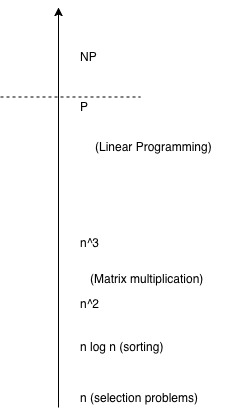
\includegraphics[scale=0.5]{img/laufzeiten}
\end{center}


\subsection{Complexity Analysis of Algorithms: time/space}
\subsubsection{Bubble-Sort}

Array: after (i+1)-step, maximum in A[1...n-i-1]

\begin{verbatim}
Bubblesort(A[1..n])
    for(i=1...n)
        for(j=1...n-i)
            if(A[j+1]<A[j])
                swap(A[j+1],A[j])
\end{verbatim}
Complexity: $\mathcal{O}(n^2)$

\subsection{Space complexity analysis}
Given Graph:
\begin{center}
	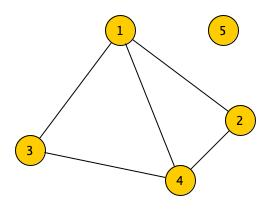
\includegraphics[scale=0.5]{img/graph1}
\end{center}

\subsubsection{Adjacency list}
\begin{center}
	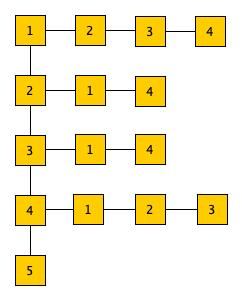
\includegraphics[scale=0.5]{img/adjL1}
\end{center}

Graph has $n$ vertices, $m$ edges. Space requirement: $\mathcal{O}(n \cdot m) \Rightarrow $ Overestimation, holds for full graph, correct answer is $\mathcal{O}(n + m)$.

\subsubsection{Adjacency matrix}

$$\begin{pmatrix}
0 & 1 & 1 & 1 & 0 \\
1 & 0 & 0 & 1 & 0 \\
1 & 0 & 0 & 1 & 0 \\
1 & 1 & 1 & 0 & 0 \\
0 & 0 & 0 & 0 & 0 \\
\end{pmatrix}$$

Entry A[i,j] = 1, if $(i,j) \in E$. On diagonal we see self loops (1). Simple graph has 0s on diagonal. Space requirements: $\mathcal{O}(n^2)$, cause matrix is $ n \times n $ big.

\subsection{Lower bounds}

\paragraph{Input} Array A[1..n]

\paragraph{Output} An Array in sorted form \\

$\exists$ algorithm that sorts in $\mathcal{O}(n\log n)$ time. \paragraph{Question} Can we do better? $\Leftrightarrow \exists$ algorithm to solve the problem in $o(n\log n)$

\fbox{\parbox{\linewidth}{\textbf{Remember:} \\
\begin{itemize}
\item $f = \mathcal{O}(g)$ upper bound $\Leftrightarrow \exists c>0 \exists x_0>0: f(x) \leq c  \cdot g(x) \forall  x \geq x_0$
\item $f = \Omega(g)$ lower bound $\Leftrightarrow \geq$
\item $f = o(g)$ strict upper bound $\Leftrightarrow <$
\item $f = \Theta(g) \Leftrightarrow f = \mathcal{O}(g) \land f = \Omega(g)$
\end{itemize}
}}
Answer: No! Sorting is in $\Omega(n \log n)$. We can simulate any algorithm that sorts an array using comparisons with a decision tree. 

\subsubsection{Example}
A[1],A[2],A[3]. 
\begin{center}
	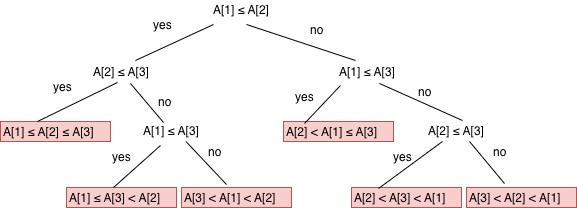
\includegraphics[scale=0.5]{img/decisiontree1}
\end{center}
$\Rightarrow$ We have n numbers, so $\#leaves = n! ( = \#permutations) \Rightarrow$ height of decision tree $\geq \log(n!) = \log(1 \cdot  2 \cdot ...\cdot n/2) \cdot ...) \geq \log(n/2)^{n/2} = \mathcal{O}(n \log n) \Rightarrow $ we need at least $\log(n!)$ comparisons.

\subsection{Mergesort}
\begin{verbatim}
MergeSort(A,l,r)
    if(l = r)
        return A[l]
    m = roundDown((l+r)/2)
    A1 = Mergesort(A,l,m)
    A2 = Mergesort(A, m+l, r)
    B = merge(A1,A2) // O(r-l)
    return B
\end{verbatim}

$$T(n) = \begin{cases} T(\lfloor\frac{n}{2}\rfloor) + T\left( \lceil\frac{n}{2} \rceil\right) + cn & n > 1 \\ 1 & n = 1\end{cases}$$ 
\begin{align*}
n = 2^k \\
T(n) &= 2 T(\frac{n}{2}) + cn  \\
&= 2 (2T(\frac{n}{2^2})+ c \frac{n}{2}) + cn \\
&= ... \\
&= 2^kT(\frac{n}{2^k})+k\cdot c \cdot n = 2^{\log n} T(\frac{n}{2^{\log n}})+ c \cdot \log n \\
&= \mathcal{O}(n \log n)
\end{align*}
With that we have proven, that sorting is in $\Theta(n \log n)$.

\subsection{Convex hull (in computational complexity)}
\paragraph{Input} Points in $\mathbb{R}^2$: $p_1 = (x_1,y_1),...$ 
\paragraph{Output} find a polygon (the smallest one) containing $p_1,...p_n$ \\
$\exists$ many algorithms that solve convex hull in $\mathcal{O}(n \log n)$ time! But: Can we do better = Can we solve the problem in $o(n \log n)$? \\
\paragraph{Idea} CH $\leq o(n \log n)$ sorting (CH is reduced to sorting in the less than $\mathcal{O}(n \log n))$ \\
Instance: $x_1,x_2,...,x_n$ to be sorted. $\Rightarrow$ CH-instance $(x_1,x_1^2),(x_2,x_2^2),...,(x_n,x_n^2)$ (all of them are in CH). The order that appear on CH is a sorting of them (CH-instances drawn look like an exponential function, if sorted by first component). <br>
if CH = $o(n \log n) \Rightarrow$   Sorting = $o(n \log n) \Rightarrow$  that doesn't work with $\Omega(n \log n)$.


\subsection{Example Recursions}

\begin{align*}
	T(n) &= 2 T(\sqrt{n}) + \log n & | m = \log n \\
	T(2^m)&= 2 T(2^{m/2}) + m & | S(m) = T(2^m) \\
	S(m) &= 2 S\left(\frac{m}{2}\right) + m & | \text{from before} \\
	& \in \mathcal{O}(m \cdot \log m) = \mathcal{O}(\log n \cdot \log \log n)
\end{align*}
\begin{align*}
T(n) &= 3T\left(\frac{n}{4}\right)+n \\
&= 3 \left(3 T\left(\frac{n}{16}\right)+\frac{n}{4}\right) +n \\
&= 3^2 T\left(\frac{n}{4^2}\right) + \frac{3}{4}n + n \\
&= 3^2 T\left(3 T \left(\frac{n}{4^3}\right)+\frac{n}{4^3}\right)+ \frac{3}{4}n + n \\
&= 3^3 T\left(\frac{n}{4^3}\right) + \frac{3^2}{4^2}n + \frac{3}{4}n + n \\
&= c \cdot 3^{\log_4(n)} + n \cdot \sum_{i=0}^{\log_4 n-1}\left(\frac{3}{4}\right)^i & | \sum_{i=0}^{\infty} q^i \stackrel{(q<1)}{\rightarrow} \frac{1}{1-q}\\
& \leq  n^{\log_4 3} + n \cdot \frac{1}{1-\frac{3}{4}} & | a^{\log_b n} = n^{\log_b a}; n^1 > n^{\log_43} \\
&= o(n) + 4\cdot n = \mathcal{O}(n)
\end{align*}

\subsection{Logarithmic rules}
\begin{enumerate}
\item $\log a^b = b \log c$
\item $\log(a\cdot b) = \log a+\log b$
\item $x=b ^{\log_bx}$
\item $\log_ax = \frac{\log_bx}{\log_ba}$
\end{enumerate}


\paragraph{Proof} $3^{\log_4n} = n^{\log_43}$
\begin{align*}
	&3^{\log_4n} = n^{\log_43} \\
	&\Leftrightarrow \log_4n = \log_3(n^{\log_43}) & | \text{rule 1}\\
	&\Leftrightarrow  \log_4n = \log_43 \cdot \log_3n \\
	&\Leftrightarrow  \frac{\log_4n}{\log_43} = \log_3n \\
	& \Rightarrow  \text{true with rule 4}
\end{align*}
\begin{flushright}
	$\square$
\end{flushright}

\subsection{One more recursion example}

Given: $A$, $B$, $n \times n$ matrices. $A \times B = C$ \\
Take every matrices and split it into partitions (for example quarters: $\begin{pmatrix}Q1&Q2\\\\Q3&Q4\end{pmatrix}$) but you loose some parts in $C$. But do it more often and combine solutions. For example you have $A_1,A_2,A_3,A_4$ and $B_1,B_2,B_3,B_4$ and we have the Partitions $C_1,C_2,C_3,C_4$ in our solutions matrices. We do it like we had no partitions, so we need to multiply and add the correct Partitions of $A$ and $B$:
\begin{itemize}
\item $C_1 = A_1 \cdot B_1 + A_2 \cdot B_3$
\item  $C_2 = A_1 \cdot B_2 + A_2 \cdot B_4$
\item  $C_3 = A_3 \cdot B_1 + A_4 \cdot B_3$
\item  $C_4 = A_3 \cdot B_2 + A_4 \cdot B_4$
\end{itemize}
That leads to the recursion formula (\textit{irgendwas bisschen komsich aber naja passt so in etwa}): \\

\begin{align*}
T(n) &= 8 \cdot T\left(\frac{n}{2}\right)+\mathcal{O}(n^2) \\
&= 8 \cdot\left(8 \cdot T\left(\frac{n}{2^2}\right) + c\frac{n^2}{2^2} \right) + c \cdot\frac{n^2}{2} \\
&= 8^2 \cdot T\left(\frac{n}{2^2}\right) + c \cdot\frac{8}{2^2}n^2 + c \cdot n^2 \\
&= 8^{\log n} + c \cdot n^2 \cdot\sum_{i=0}^{\log n -1}\left(\frac{8^i}{2^{2i}}\right) & | \sum_{i=0}^{\log n -1}\left(\frac{8^i}{2^{2i}}\right) = \sum_{i=0}^{\log n -1} 2^i = 2^{\log n} -1  \rightarrow  n\\
&= n^{\log_28} + c \cdot n^2 \cdot n \\
&= n^3 +  c  \cdot n^3 = \mathcal{O}(n^3)
\end{align*}

Other way for matricemultiplication: \\
$P_1 = A_1 \cdot (B_2 - B_4)$, $P_2 = B_4 \cdot(A_1-A_2)$,...,$P_7=(A_1-A_3) \cdot (B_1 + B_2)$ \\
$C_1 = P_5 + P_4 - P_2 + P_6$, $C_2=...$,... \\
Recursion formula: $T(n) = 7 \cdot T\left(\frac{n}{2}\right) + \mathcal{O}(n^2)$, so we only have $n^{\log_27} \approx n^{2.8} < n^3$. This is called STRASSEN - schema

\subsection{Analyse complexity/costs with probabilities (average analysis)}

\begin{verbatim}
find_min(Array A)
    min = A[0] //c1
    for(i=1,...n-1)
        if(A[i] < min) //c2
        min = A[i] // c3
    return(min)
\end{verbatim}
Total costs: $c = c_1 + (n-1) \cdot c_2 + (n-1) \cdot c_3$ 

Get probabilities for doing $c_3$: 
$$P(A[1] < A[0]) = \frac{1}{2}$$
$$P(A[2] < min(A[0],A[1])) = \frac{1}{3}$$
$$P(A[i] < min(A[0],...,A[i-1])) = \frac{1}{i+1}$$
Now we can calculate the costs with these probabilities: 
$$X_i = \begin{cases}1 & if(A[i-1]< min(...)) \\\\ 0 & otherwise \end{cases}$$
$$c = c_1 + (n-1) \cdot c_2 + \sum_{i=1}^{n-1}X_i$$
$$E[X_i] = P(X_i = 1) = \frac{1}{i+1}$$
$$E\left[\sum_{i=1}^{n-1}X_i\right] = \sum_{i=1}^{n-1}E[X_i] = \sum_{i=1}^{n-1}\frac{1}{i+1} = \log n$$

\subsection{Armortised Analysis}
Stack $S$ with \texttt{PUSH(x)}($\mathcal{O}(1)$) and \texttt{POP()}($\mathcal{O}(1)$) and \texttt{MULTI-POP(k)} ($\mathcal{O}(min(|S|,k))$) operation. \\
$n$ operations: $\mathcal{O}(n^2)$ because worst operation (`MULTI-POP(k)`) is linear. That's pessimistic. \\
\subsubsection{Accountingmethod}
\begin{tabular}{|c|c|}\hline
	cost & operation \\ \hline
	2 coins & \texttt{push(x)} \\
	0 coins & \texttt{pop()} \\
	0 coins & \texttt{multi-pop(k)} \\ \hline 
\end{tabular} 

$\Rightarrow n$ opertions cost $\leq 2n \Rightarrow \mathcal{O}(n)$

if \texttt{pop()} or \texttt{multi-pop(k)} are applied, at least 1 or $k$ Elements are on the stack $\Rightarrow k$ coins are on the stack.

\subsubsection{Potentialmethod}
"function that describes the bank/the benefit one get doing cheap operations in order to do bad operations" 
\begin{itemize}
\item  $D$ Data structure
\item  $i$ step 
\item  $\Phi$ real value $\geq$ 0
\item $\hat{c_i}$ amortized cost
\item  $c_i$ cost of operation
\item $D_0 \Rightarrow \Phi(D_0) = 0$
\item $D_i (i > 0) \Rightarrow \Phi(D_i) \geq i$

\end{itemize}

$$\hat{c_i} = c_i + \Phi(D_i) - \Phi(D_{i-1})$$

\begin{itemize}
\item \texttt{push(x)} amortized: $1 + |S| + 1 - |S| = 2$
\item  \texttt{pop()} amortized: $1 + |S| - 1 - |S] = 0$
\item  \texttt{multi-pop(k)} amortized: $min(|S|,k) + |S| - min(|S|,k) - |S| = 0$
\end{itemize}

$$\sum_{i=1}^n \hat{c_i}= \sum_{i=1}^n (c_i + \Phi(D_i) - \Phi(D_{i-1}) = \sum_{i=1}^n c_i + \sum_{i=1}^n (\Phi(D_i)-\Phi(D_{i-1})) = \sum_{i=1}^n c_i + \Phi(D_n) [\geq0] - \Phi(D_0)[=0]$$

